\documentclass[12pt,titlepage,french]{article}
\usepackage{babel}
\usepackage{graphicx}
\usepackage[margin=2.5cm]{geometry}

\usepackage[hidelinks]{hyperref}
\usepackage{tabularx}
\usepackage{float}
\usepackage[utf8]{inputenc}
\usepackage[T1]{fontenc}
\pagestyle{plain}

\usepackage{booktabs,makecell,tabu}
\usepackage{comment}
\renewcommand\theadfont{\bfseries}

\linespread{1.5}

\newcounter{firstbib}

\begin{document}
%\renewcommand{\thesection}{\arabic{section}} % utilisé pour spécifier la numérotation des sections

\begin{titlepage}
\newcommand{\HRule}{\rule{\linewidth}{0.5mm}}
\center

  
\includegraphics[width=0.45\textwidth]{../../ressources/img_logos/logo_polytech.png}\\[1cm]

  
\includegraphics[width=0.45\textwidth]{../../ressources/img_logos/logo_taglabs.png}


\HRule \\[0.4cm]
{ \huge \bfseries Rapport itération 5\\[0.15cm] }
Classification colorimétrique de nuages de points 3D\\
Version 1.0\\
Le \today \\
\HRule \\[1.5cm]
Ronan Collier,
Mathieu Letrone,
Tri-Thien Truong
\\[1cm]
\end{titlepage}

\tableofcontents % table des matières
\newpage
\listoffigures  % table des figures
\newpage

\section{Rappel des objectifs de l'itération}
Suite à l'itération où nous avions amélioré notre solution, nous avons voulu élargir nos types de filtrages, en utilisant d'autres espaces colorimétriques. De plus, nous avions encore des tâches en cours, que nous devions avancer/finaliser.

Durant l'itération précédente, nous avons pu implémenter un nouveau filtre, en utilisant l'espace colorimétrique HSV. Il nous fallait maintenant avoir des retours clients pour que l'on puisse corriger les différents bugs. De plus, des tâches majeures étaient encore en cours.

Les tâches que nous nous sommes fixées sont les suivantes :

\begin{itemize}
    \item Restreindre l'utilisateur lors de la saisie du filtrage RGB (borne inférieure et supérieure)
    \item Amélioration des plages du filtrage HSV + test de performance
    \item Résoudre les divers problèmes techniques qui empêchent le fonctionnement de l'algorithme de segmentation
    \item Résoudre problèmes et débuggage du tone mapping
    \item Comparer les performances avec un autre algorithme de tone mapping
\end{itemize}

Nous avions aussi une tâche qui s'est ajoutée pendant l'itération, qui était d'exporter le plugin pour pouvoir l'utiliser sur toutes les machines, en utilisant CloudCompare. Nous avions aussi eu des retours utilisateurs, afin d'améliorer notre plugin.

\section{Production / réalisation durant l'itération}

Nous développerons ici chaque objectif que nous nous sommes fixé pour cette itération.


\subsection{Exportation du plugin}

Dans le but d'avoir des retours de notre client, nous avons voulu exporter notre plugin pour qu'il soit utilisable avec le logiciel CloudCompare, sur une machine quelconque. \newline

Pour ce faire, le principe est de récupérer le fichier ColorimetricSegmenter.dll que nous obtenons lorsque nous compilons le projet, et de l'intégrer dans le dossier "plugins" dans le répertoire d'installation de CloudCompare. \newline

Nous avons rencontrés des difficultés lors de cette tâche. En effet, nous avons vu qu'il y avait des problèmes de versions des dépendances, qui ne faisaient pas fonctionner notre plugin sur toutes les machines. \newline

En effet, lorsque nous compilions notre projet, nous utilisions Visual Studio 2019. En utillisant cette version, la version du windows SDK était aussi modifiée, et c'était la source du problème de compatibilité entre nos machines, qui avaient une version de windows plus récente que les machines de notre client, ou encore M. Daniel Girardeau-Montaut, le créateur de CloudCompare.

\begin{figure}[H]
 \caption{\label{} Notre version du SDK Windows, avec Visual Studio 2019}
 \begin{center}
 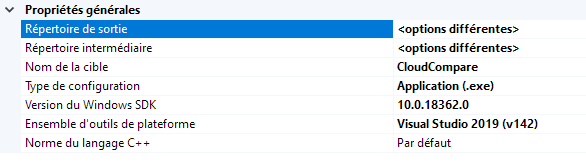
\includegraphics[width=1\textwidth]{./img/vs2019.PNG}
  \end{center}
\end{figure}


\begin{figure}[H]
 \caption{\label{} Version du SDK Windows correcte, avec Visual Studio 2017}
 \begin{center}
 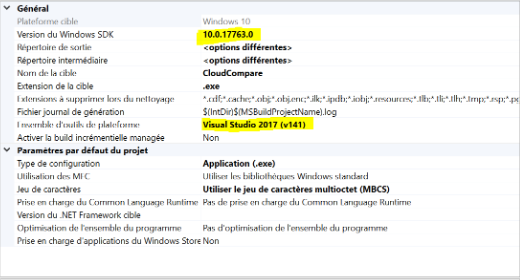
\includegraphics[width=1\textwidth]{./img/vs2017.PNG}
  \end{center}
\end{figure}

Grâce à cette solution, le client a pu tester notre plugin de son côté, et a pu nous faire des retours concrets sur l'utilisation de notre plugin.

\subsection{Restreindre l'utilisateur lors de la saisie du filtrage RGB}

Lorsque nous avons décidé cette tâche, nous voulions améliorer le filtrage RGB côté utilisateur, afin de mieux choisir les bornes minimum et maximum. \newline

En effet, l'utilisation de l'espace colorimétrique RGB limite les bornes que l'on peut utiliser, afin de sélectionner les points que l'on veut. Pour que ce filtrage fonctionne correctement, nous sommes obligés de sélectionner deux points qui ont la même gamme de couleurs. Il faut ensuite choisir le point le plus "sombre", c'est-à-dire avec les valeurs RGB les plus faibles, puis le point le plus clair. \newline

Plusieurs problèmes peuvent se poser. Par exemple, si l'utilisateur décide de prendre des points dans des gammes de couleurs différentes, ce qui donne un résultat non satisfaisant. Il peut aussi avoir un problème lorsque l'utilisateur inverse la sélection des points, ce qui inverse les bornes. Il n'y aurait donc aucun point de sélectionné. \newline

Une solution peut consister à inverser les valeurs, si l'utilisateur se trompe. Pour cela, il faut être sûr que l'utilisateur a bien choisi deux points de la même gamme de couleur, puis vérifier que les trois composantes du deuxième point sont inférieures au premier point, afin de les inverser. \newline

Une question reste en suspend, qui est de savoir si nous réalisons le traitement directement sur l'interface (l'utilisateur verra donc directement le changement des bornes), ou si le traitement se fera au niveau en prétraitement du parcours de points, et l'utilisateur aura juste à choisir ses deux points. \newline

Après réunion, le choix qui a été fait est de faire un traitement caché à l'utilisateur, afin de créer les bornes. Pour faire cela, il faudra donc savoir lequel des deux points sélectionnés, est le plus foncé et le plus clair. \newline

En restant sur l'espace colorimétrique RGB, il semble assez difficile de le savoir. C'est pour cela que nous pensons passer par le HSV (conversion déjà réalisée) pour utiliser la composante "Value", qui nous donnera le point le plus sombre (Value proche de 0), et le point le plus clair (proche de 100). \newline

Dans le cas où la Value est la même, nous pourrions alors passer par la saturation, où le point le plus clair sera le point où sa saturation est la plus faible. \newline

Enfin, dans le cas où les 2 composantes ont les mêmes valeurs, c'est que la teinte est différente. Ici, nous pourrions prendre les valeurs minimums entre les 2 composantes en RGB les plus faibles (c'est-à-dire, ne pas prendre en compte la composante dominante, mais les deux autres), afin de faire la borne inférieure, puis inversement pour la borne supérieure. Ici, on considérera donc que l'utilisateur choisira des points qui ont la même teinte de couleur, ou des teintes très similaires.

\subsection{Amélioration des plages du filtrage HSV}

Grâce aux retours utilisateurs, nous avons pu améliorer notre filtrage HSV, mais aussi le filtrage RGB, au niveau de l'interface. En effet, nous avons pu remarquer qu'il y avait un problème notamment au niveau de la redimension de la fenêtre de l'interface. Il fallait ajouter certains layouts/spacers, pour que nos différents éléments s'adaptent en fonction de la taille de la fenêtre. 

Par exemple, nos fenêtres avaient des problèmes sur un écran 4k, car elles étaient trop petites.

\begin{figure}[H]
 \caption{\label{} Fenêtre RGB sur écran 4k}
 \begin{center}
 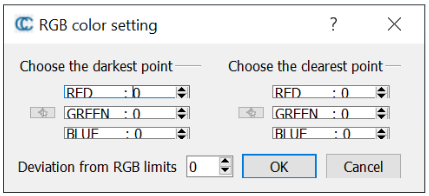
\includegraphics[width=0.6\textwidth]{./img/rgb_pb.PNG}
  \end{center}
\end{figure}

Nous avons donc dû repasser sur nos fenêtres, et les refaire proprement afin de mettre des layouts aux bons endroits, et des spacers entre les éléments pour qu'ils s'adaptent bien selon la taille totale de la fenêtre.

\begin{figure}[H]
 \caption{\label{} Nouvelle fenêtre, taille petite}
 \begin{center}
 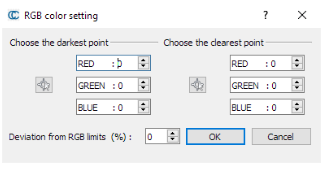
\includegraphics[width=0.8\textwidth]{./img/rgb_new1.PNG}
  \end{center}
\end{figure}

\begin{figure}[H]
 \caption{\label{} Nouvelle fenêtre, grande taille}
 \begin{center}
 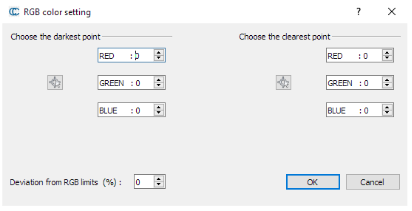
\includegraphics[width=1\textwidth]{./img/rgb_new2.PNG}
  \end{center}
\end{figure}

De plus, nous avons revu l'algorithme pour effectuer la conversion des valeurs RGB en HSV. En effet, nous effectuions la conversion au moment de la sélection d'un point, donc après le point picking. Ce fonctionnement pouvait poser problème notamment lorsque l'utilisateur voulait rentrer à la main ses valeurs de RGB. Il fallait donc revoir l'action qui allait lancer le processus de conversion. \newline

Pour faire cela, nous avons décidé de lancer la conversion lorsqu'un des trois champs RGB était modifié. Comme ça, l'utilisateur pourra mettre à la main ses valeurs, pour actualiser les valeurs HSV, ou passer par le point picking, qui va actualiser les valeurs RGB, et donc automatiquement actualiser les valeurs HSV. \newline

Dans un souci d'optimisation, au lieu d'actualiser trois fois les valeurs au moment du point picking (car les 3 champs RGB sont actualisés en même temps), nous réalisons qu'une seule actualisation.

\begin{figure}[H]
 \caption{\label{} Fenêtre HSV, actualisation manuelle}
 \begin{center}
 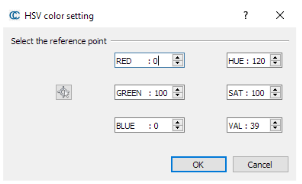
\includegraphics[width=0.7\textwidth]{./img/hsv.PNG}
  \end{center}
\end{figure}

\subsection{Algorithme de segmentation}


L'algorithme de segmentation n'est toujours pas fonctionnel. Ce retard est dû à la difficulté de débogage de CloudCompare. L'exécution de l'algorithme provoque un arrêt de l'application. Les erreurs retournées sont très peu explicites et ne permettent pas de savoir la cause du problème (erreur de segmentation par exemple). \newline

De multiples actions dans l'algorithme nécessitent la manipulation de structures de données complexes, ce qui donne également lieu à bon nombre d'erreurs. Par exemple, en parcourant le nuage de points afin de regrouper les points sous forme de régions de plus proches voisins. Afin de réaliser cela, nous utilisons la structure "Octree". Elle dispose de plusieurs méthodes permettant la recherche rapide de voisins. Cependant, l'implémentation de cette structure reste parfois opaque et nécessite un certain temps de prise en main. \newline

L'algorithme nécessite de créer plusieurs fois des sous-nuages de points afin de constituer des régions. Pour des raisons de rapidité, nous ne recopions pas à chaque fois le nuage de point, mais nous utilisons plutôt la structure "ReferenceCloud" qui contient les références des points présents dans le nuage de point d'origine. L'inconvénient de cette structure réside dans l'utilisation simultanée de deux types d'index : les index globaux (ceux du nuage de point d'origine) et les index locaux (du nuage par référence). Cela donne lieu à de multiples confusions dans l'algorithme.\newline

Le débogage du plugin se poursuivra lors de la prochaine itération.

\subsection{Tone Mapping}

À la fin de l'itération précédente, une première version de l'algorithme basé sur la segmentation de l'histogramme était implémentée, hélas, elle restait non opérationnelle. Une fois le processus lancé, le logiciel CloudCompare cessé de fonctionner. Ainsi, dans cette itération, il fallait déterminer la cause de problème et y remédier.

Après plusieurs refontes de la structure de l'algorithme et d'une phase de débuggage laborieuse, la fonctionnalité fonctionne. Le problème venait du non support de CloudCompare de méthodes d'itérateurs des map de la libraire standard.

Son utilisation est comme suit, l'utilisateur sélectionne le ou les nuages sur lesquels il veut appliquer le tone mapping. Une fenêtre de dialogue apparaît lorsqu'il clique sur "Histogramme clustering"

\begin{figure}[H]
 \caption{\label{} Fenêtre de dialogue Tone mapping}
 \begin{center}
 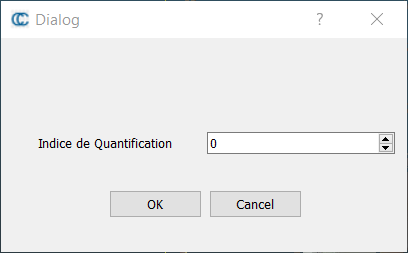
\includegraphics[width=0.4\textwidth]{./img/ToonMappingDialog.PNG}
  \end{center}
\end{figure}

L'utilisateur indique l'indice de quantification souhaité et lance l'algorithme. Une fois le processus fini, le sous-scan résultant est affiché. Les images suivantes illustrent les résultats obtenus avec différents indices saisis.
\begin{figure}[H]
 \caption{\label{} Exemples du Tone Mapping}
 \begin{center}
 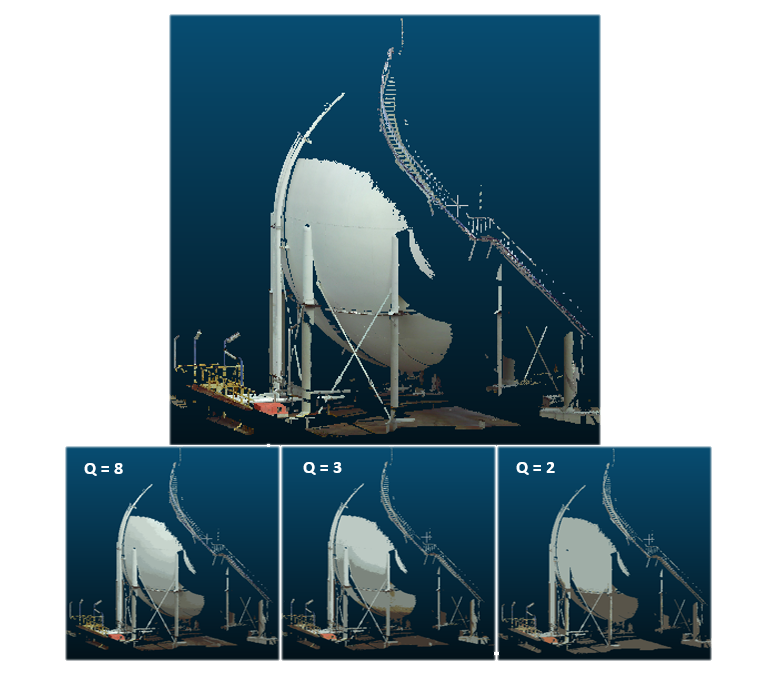
\includegraphics[width=0.8\textwidth]{./img/ExpToonMapping.PNG}
  \end{center}
\end{figure}
Pour un Q donné, on aura une palette de $Q^2$ couleurs dans le nuage résultat.\newline

En plus de rendre opérationnel cet algorithme, un autre algorithme de tone mapping devait être implémenté afin de pouvoir comparer les performances desdits algorithmes. Malheureusement, du retard a été pris, son implémentation est bien avancée mais n'est pas terminée. Cet Algorithme basé sur la classification k-means, qui permettra d'avoir k groupes de couleur une fois le

\section{Risques éliminés durant l'itération}

Pour cette itération, nous avons corrigé de nombreux bugs plus ou moins critiques, ce qui nous a permis d'avoir un plugin beaucoup plus stable. Il nous reste encore certains bugs à corriger, que nous avons eu grâce au feedback.

\section{Feedback}

Durant cette itération, le feedback nous a été très important afin de savoir que nous devions améliorer et/ou corriger. Suite à notre réunion de fin d'itération, nous avons pu mettre au clair ce qui était encore en cours, et montrer notre avancée sur le projet. Globalement, celle-ci est satisfaisant, avec quelques améliorations potentielles :

\begin{itemize}
    \item Ajouter une fonctionnalité pour choisir les points externes ou internes du filtre
    \item Améliorer l'interface sur la redimension de la fenêtre (OK)
    \item Ajouter des indications sur les interfaces, notamment les bornes pour le HSV
    \item Choisir une icône pour le plugin
\end{itemize}

Ces remarques seront pris en compte pour la prochaine itération.

\section{Commentaires sur l'itération}

Cette section va présenter nos ressentis sur notre itération. Cela peut correspondre à la façon dont nous avons pu gérer la charge de travail que nous avions prévu en début d'itération, des potentiels imprévus, points positifs/négatifs, et autres.

\subsection{Commentaires sur l'itération de façon générale}

Tout d'abord, nous avons dû replanifier notre itération, notamment à cause du coronavirus, qui a provoqué l'annulation du projet ICreate. Nous avions prévu que cette itération allait être compliqué à cause de ce projet. Avec son annulation, il nous fallait revoir notre planning, pour réaliser nos tâches sur cette itération, et la prochaine. \newline

De plus, un membre du projet a été victime de ce virus, et était dans l'incapacité de travailler. Il va maintenant mieux, et va pouvoir reprendre ses tâches. \newline

Concernant les différentes tâches, nous avons eu beaucoup de mal à cerner le problème de compatibilité de notre plugin avec les machines de notre client. En effet, comme notre plugin fonctionnait sur nos machines, le seul moyen pour trouver le problème était de le faire tester directement avec notre client. \newline

Comme notre moyen de discussion était via email, le délai entre questions et réponses, puis les tests avec les retours, était assez long. Heureusement, nous avons pu trouver une solution grâce au créateur du plugin M. Daniel Girardeau-Montaut, et nous le remercions grandement pour le temps qu'il a pu nous accorder afin de résoudre notre problème.

\subsection{Commentaires sur les méthodes de travail/changements de méthode}

Nous avons continué avec les mêmes méthodes de travail pour cette itération. Chacun a ses tâches à faire qui sont indépendantes des autres, il est donc assez facile de se répartir et que chacun avance à son rythme.

\section{Objectifs de la prochaine itération}

Pour la dernière itération, il faut finaliser les tâches qui étaient en cours, et prendre en compte le feedback pour appliquer les correctifs nécessaires :

\begin{itemize}
    \item Désactiver les filtrages si le nuage ne correspond pas (RGB => désactiver si nuage en gris)
    \item Redéfinir les bornes pour filtrage RGB
    \item Implémenter le filtrage via valeusr scalaires
    \item Réaliser les tâches du feedback (points externes/internes, indications, icône)
    \item Finir algo k-means/autre algorithme
    \item Terminer algorithme sélection de points
    \item Faire le lien entre tone mapping et filtrage
\end{itemize}
\end{document}
